\subsection{Design and Testing on Migration of Remiss-Supply in Banking System to Microservice Architecture \cite{maulana_design_2022}}

\label{subsec:maulana_design}

\textcite{maulana_design_2022} apresentam um estudo focado na migração arquitetural de um sistema bancário monolítico para uma arquitetura de microsserviços, especificamente para o serviço de Remiss Supply do PTBank Indonesia. A principal motivação para a migração, conforme destacado pelos autores, reside na superação das limitações das arquiteturas monolíticas tradicionais, que apresentam falta de flexibilidade, dificuldades de manutenção e suscetibilidade a falhas em cadeia.

Foram utilizados como base do estudo os subserviços do sistema proprietário Remiss Supply, descritos pelo pesquisador em seu trabalho e visíveis na ilustração \autoref{fig:3-maulana-scenario}. Os três sistemas analisados foram:

\begin{itemize}
    \item \textbf{Inquiry Data}: Responsável por realizar buscas e consultas de dados completos de transações históricas, permitindo o rastreamento de atividades de depósito e retirada com base em parâmetros como datas de recebimento, entrega, identificação da agência e ID da transação;
    
    \item \textbf{Inquiry Details}: Especializado em fornecer informações detalhadas e específicas sobre transações, incluindo denominações de cédulas e dados complementares que aprofundam a análise das operações realizadas;
    
    \item \textbf{Remis Supply Request}: Gerencia solicitações de novas transações de retirada e depósito, processando casos de "REMIS" (depósitos em numerário) e "SUPPLY" (retiradas em numerário), incluindo validações, conexões com serviços centrais e persistência de dados transacionais;
\end{itemize} 

O processo de migração do serviço do banco foi segmentado em sprints, com foco na análise do sistema monolítico, no design do banco de dados, na coleta de recursos, na criação de esquemas \gls{xml} para requisições e respostas, e na implementação do código para os microsserviços. Por fim, realiza-se a implantação em contêineres Docker\footnote{Disponível em https://www.docker.com/} e máquinas virtuais, utilizando a linguagem de programação Java\footnote{Disponível em https://www.java.com/} na implementação.

\begin{figure}
    \caption{Cenário descrito nos testes}
    \label{fig:3-maulana-scenario}
    \centering
    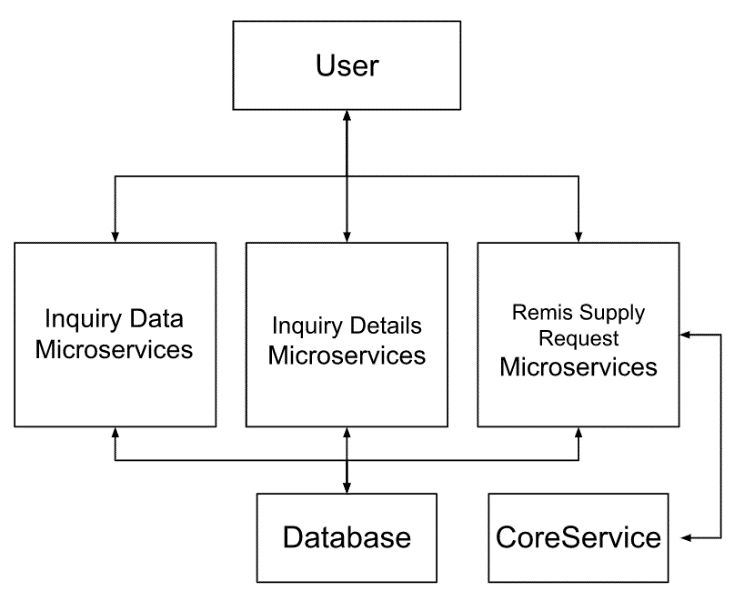
\includegraphics[width=0.5\linewidth]{imagens/maulana_scenario.jpg}    
    {\par \raggedright \footnotesize Fonte: \textcite{maulana_design_2022}.\par}
\end{figure}

Os testes de desempenho foram realizados para comparar as arquiteturas monolítica e de microsserviços sob diferentes condições de carga e estresse, incluindo variações no número de requisições simultâneas e cenários de alta (Ver \autoref{tab:3-maulana-testes-carga}) concorrência, utilizando o tempo de resposta, a latência e o \textit{throughput} como métricas principais. 

\begin{table}[H]
\centering
\caption{Condições de carga e estresse}
\label{tab:3-maulana-testes-carga}
\makebox[\textwidth][c]{%
\begin{tabularx}{\textwidth}{|l|X|}
\hline
\textbf{Condições de carga} & Throughput de 200 e 1.000 threads por minuto. \\
\hline
\textbf{Condições de estresse (microsserviços)} & \textit{Ramp-up} de 1 a 1.000 threads. \\
\hline
\end{tabularx}%
}
{\par \raggedright \footnotesize Fonte: \textcite{maulana_design_2022}.\par}
\end{table}

Na arquitetura monolítica, os resultados revelaram tempos distintos entre os subserviços: o serviço Remis Supply Request apresentou o maior tempo médio de resposta, de \textbf{1.616,06 ms}, devido à sua complexidade operacional, já mencionada no detalhamento dos serviços. Em seguida, o Inquiry Data registrou \textbf{389,65 ms} e o Inquiry Details, \textbf{241,175 ms}, como pode ser observado nas figuras \ref{fig:maulana_thp_mono} e \ref{fig:maulana_time_mono}. A latência e o \textit{throughput} variaram conforme a complexidade do fluxo de cada subserviço, impactando diretamente o desempenho do sistema monolítico.



\begin{figure}[htb]
  \centering
  \begin{minipage}[t]{0.48\linewidth}
    \caption{Throughput Cenário Monolítico}
    \label{fig:maulana_thp_mono}
    \centering
    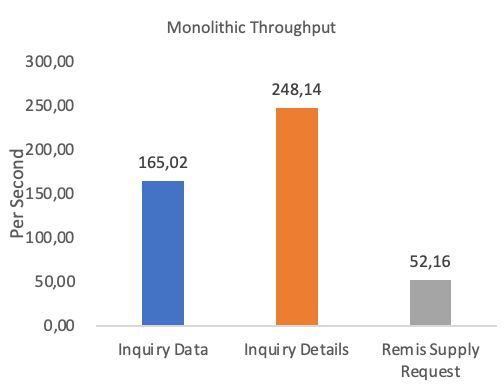
\includegraphics[width=\linewidth]{imagens/maulana_thp_mono.jpg}    
    {\par \raggedright \footnotesize Fonte: \textcite{maulana_design_2022}.\par}
  \end{minipage}%
  \hfill
  \begin{minipage}[t]{0.48\linewidth}
    \caption{Throughput Cenário Microsserviços}
    \label{fig:maulana_thp_ms}
    \centering
    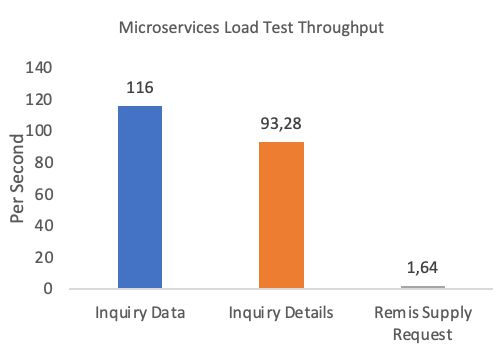
\includegraphics[width=\linewidth]{imagens/maulana_thp_ms.jpg}
    
    {\par \raggedright \footnotesize Fonte: \textcite{maulana_design_2022}.\par}
  \end{minipage}
\end{figure}

Em contraste, nos testes com a arquitetura de microsserviços, os tempos de resposta evidenciam diferenças significativas. O subserviço Remis Supply Request apresenta o maior tempo de resposta médio, de \textbf{4.240,4 ms}, superando consideravelmente o Inquiry Data, que registra \textbf{586 ms}, e o Inquiry Details, que alcança \textbf{552 ms} conforme ilustrado nas figuras \ref{fig:maulana_thp_ms} e \ref{fig:maulana_time_ms}. Os subserviços Inquiry Data e Inquiry Details demonstram resultados instáveis, com variações de desempenho e tendem a diminuir sob alta carga, sugerindo desafios na orquestração e na comunicação entre os novos serviços.

\begin{figure}[htb]
  \centering
  \begin{minipage}[t]{0.48\linewidth}
    \caption{Latência Cenário Monolítico}
    \label{fig:maulana_time_mono}
    \centering
    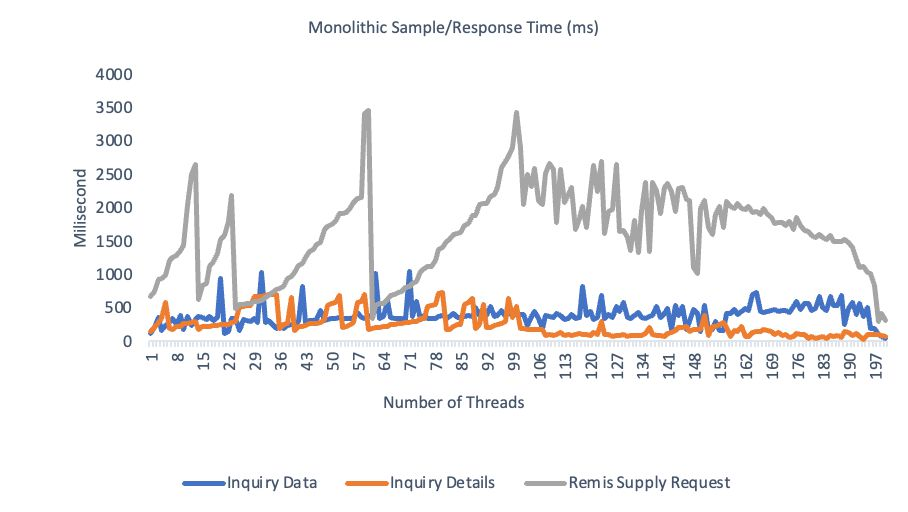
\includegraphics[width=\linewidth]{imagens/maulana_time_mono.jpg}    
    {\par \raggedright \footnotesize Fonte: \textcite{maulana_design_2022}.\par}
  \end{minipage}%
  \hfill
  \begin{minipage}[t]{0.48\linewidth}
    \caption{Latência Cenário Microsserviços}
    \label{fig:maulana_time_ms}
    \centering
    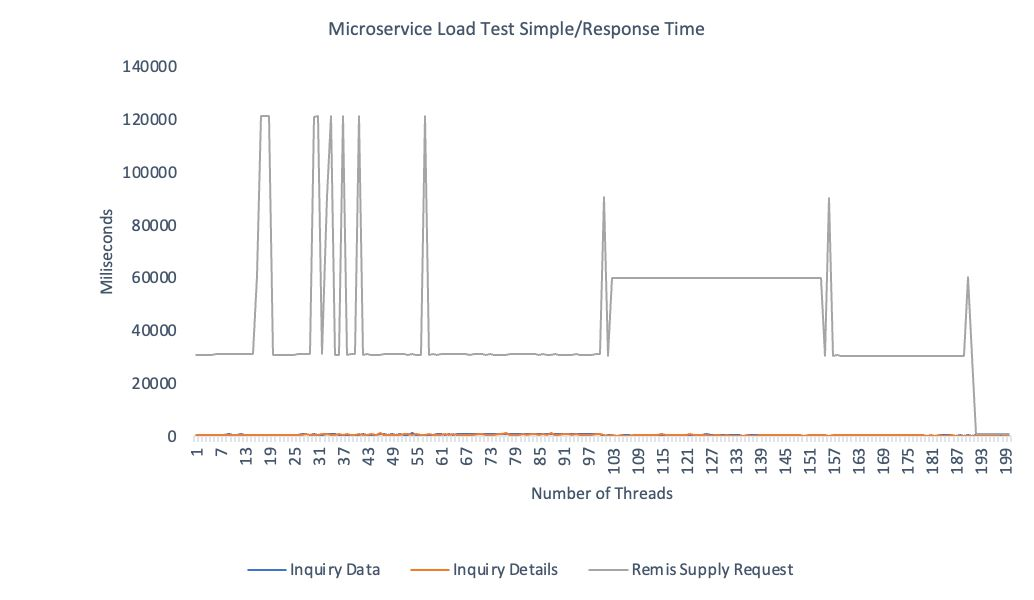
\includegraphics[width=\linewidth]{imagens/maulana_time_ms.jpg}    
    {\par \raggedright \footnotesize Fonte: \textcite{maulana_design_2022}.\par}
  \end{minipage}
\end{figure}

Além dos testes de carga, foram realizados cenários de stress testing para avaliar a capacidade da arquitetura de microsserviços em lidar com grandes volumes de requisições simultâneas. Os autores concluíram que, embora a arquitetura monolítica, executada em servidor on-premises (Intel® Xeon® CPU E5-2680 v3 @ 2.50GHz, 8GB \acrshort{ram} com Docker), tenha apresentado melhor desempenho em alguns testes específicos de tempo de resposta, a arquitetura de microsserviços, hospedada em máquina virtual no Google Compute Engine (n1-standard-2, Intel Haswell 1 vCPU, 7.5GB \acrshort{ram}) com Spring Boot, é preferível para desenvolvimento e manutenção. Isso decorre da simplicidade de gerenciamento, independência entre os subserviços e possibilidade de uso de diferentes tecnologias conforme a necessidade, aspectos inviáveis na arquitetura monolítica \cite{rademacher_modeling_2020}.

 \subsubsection{Resumo do Estudo}

Em síntese, o estudo de \textcite{maulana_design_2022} investigou a migração de um sistema bancário monolítico para microsserviços, com foco nos testes de desempenho em um contexto financeiro real. A pesquisa avaliou métricas como tempo de resposta, latência e \textit{throughput} em cenários de carga e estresse, destacando a capacidade dos microsserviços de atender às demandas de robustez e adaptabilidade do setor bancário. Os resultados indicaram que, embora o desempenho bruto em alguns testes específicos possa favorecer o sistema monolítico, em função das diferentes especificações de hardware utilizadas nos experimentos, a arquitetura de microsserviços é considerada superior para o desenvolvimento e a manutenção, devido à modularidade e à flexibilidade tecnológica. Essas características são cruciais para a agilidade e a inovação exigidas por bancos e outras instituições financeiras.

Contudo, uma limitação significativa do trabalho reside no fato de que os autores não investigaram diferentes formas de orquestração de microsserviços, focando exclusivamente na comparação entre arquiteturas monolítica e de microsserviços. Essa lacuna é particularmente relevante, pois a escolha do protocolo de comunicação entre microsserviços (\gls{rest}, \gls{grpc}, Apache Thrift, entre outros) pode impactar substancialmente o desempenho, a latência e a eficiência operacional do sistema, aspectos críticos para aplicações bancárias que demandam alta disponibilidade e tempos de resposta consistentes. A ausência de uma análise comparativa entre diferentes tecnologias de orquestração constitui uma oportunidade de pesquisa importante para aprofundar a compreensão sobre como otimizar a comunicação inter-serviços em ambientes financeiros distribuídos, reforçando a relevância da presente pesquisa no contexto da transformação digital do setor financeiro.
